\section{Method}
\label{method}

This section introduces the design of our unified tokenizer and explains how its dual visual codebooks are utilized within the next-token prediction paradigm for multimodal understanding and generation.

\subsection{Motivation and Verification}
\label{sec:motivation}

\begin{minipage}[t]{0.389\textwidth}
    As discussed in \citet{qu2024tokenflow}, CLIP encoders cluster images by semantic similarity, whereas VQVAE-based encoders group images by low-level attributes such as color and texture. This suggests that encoders trained for reconstruction primarily capture low-level visual appearance, while those trained with text alignment excel at capturing high-level semantics. We argue that this difference in representation space is a key factor underlying downstream MLLM performance. Yet such a claim has not been formally validated before.
\end{minipage}
\hfill
\begin{minipage}[t]{0.598\textwidth}
\vspace{-0.25cm}
    \centering
    \captionsetup{type=table}
    \caption{
        \textbf{Downstream visual understanding performance with different vision encoders within the LLaVA-1.5 framework.} The \textit{CLIP-based} encoder corresponds to the siglip-so400m-14-384 model~\citep{alabdulmohsin2023so400m}, whereas \textit{CLIP-based (recon.)} denotes an encoder with the same architecture but trained solely for reconstruction from scratch, controlling for factors like model size and architecture. For the \textit{VQVAE-based} encoder, we adopt SBER-MoVQGAN-270M, a well-established reconstruction model.
    }
    \label{tab:validation}
    \vspace{-0.1cm}
    \resizebox{\linewidth}{!}{
    \tablestyle{3pt}{1.12}
    \begin{tabular}{l|cccc|cc}
    \toprule
    Vision Encoder Type       &MMB\higherbetter &MME\higherbetter                     &SEED\higherbetter  &VQAv2\higherbetter     &Zero-Shot\higherbetter    &rFID\lowerbetter       \\
    \midrule
    CLIP-based &61.8                 &1492.9                   &58.4                   &78.5       & 83.2&          \textcolor{red}{\ding{55}}\\
    
    CLIP-based (recon.)     &36.2&822.4&30.6& 47.5&\textcolor{red}{\ding{55}}&0.96\\
    
    VQVAE-based     &35.8&792.0&34.1& 45.2&\textcolor{red}{\ding{55}}&0.68\\
  \bottomrule
  \end{tabular}}
\end{minipage}

To validate this viewpoint, we started by a preliminary experiment following the LLaVA-1.5 pipeline~\citep{liu2024llava1d5}.
In Table.\ref{tab:validation}, compared to the original SigLIP model, encoders trained with reconstruction objective exhibit a significant drop in downstream MLLM vision-language understanding performance, validating that high-level semantic features are more critical for visual reasoning in MLLMs than low-level perceptual features.
However, to achieve both visual understanding and generation within a single MLLM, it is essential to decode the visual tokens back into pixel space as accurately as possible. However, since the SigLIP encoder focuses on high-level semantic information rather than texture details, simply discretizing its features and training a decoder without tuning the encoder results in poor image reconstruction quality. % as shown in Fig.~\ref{}. 
Therefore, proposing a unified tokenizer is crucial to enable high-quality visual understanding and generation within a singe MLLM.


\begin{figure*}[t]
  \centering
  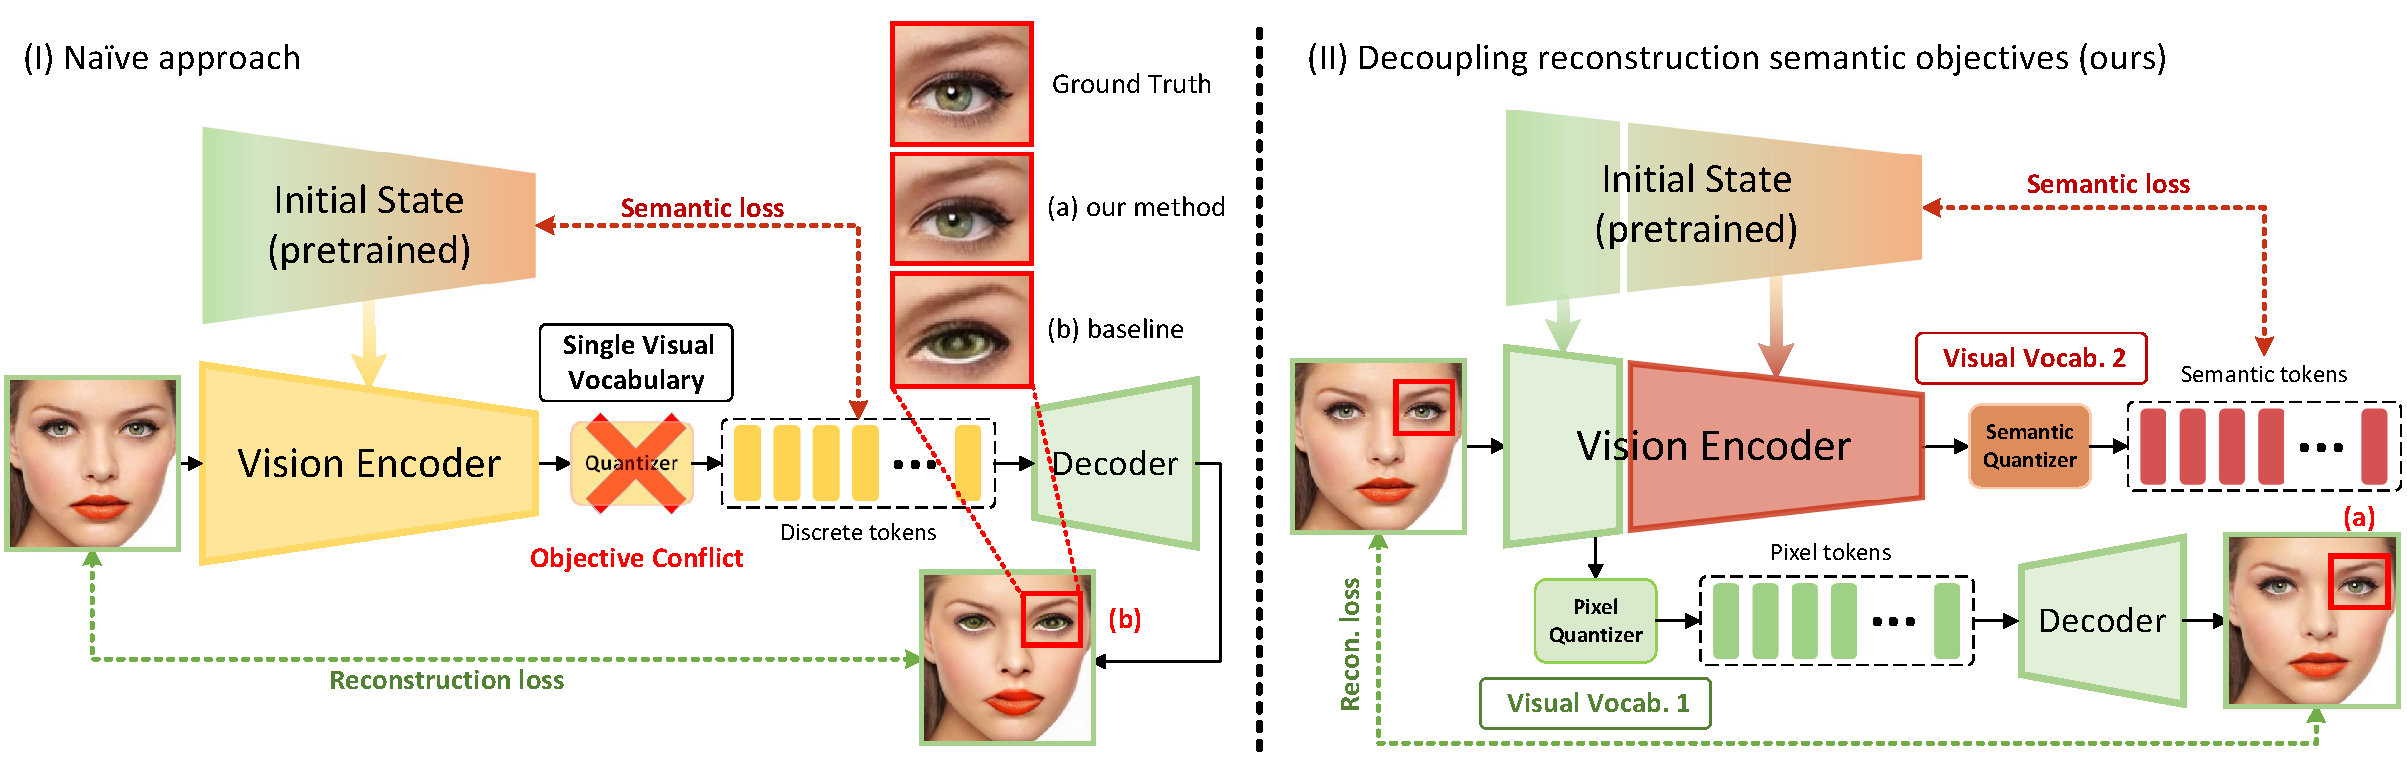
\includegraphics[width=0.92\textwidth]{imgs/tokenizer.pdf}
  % 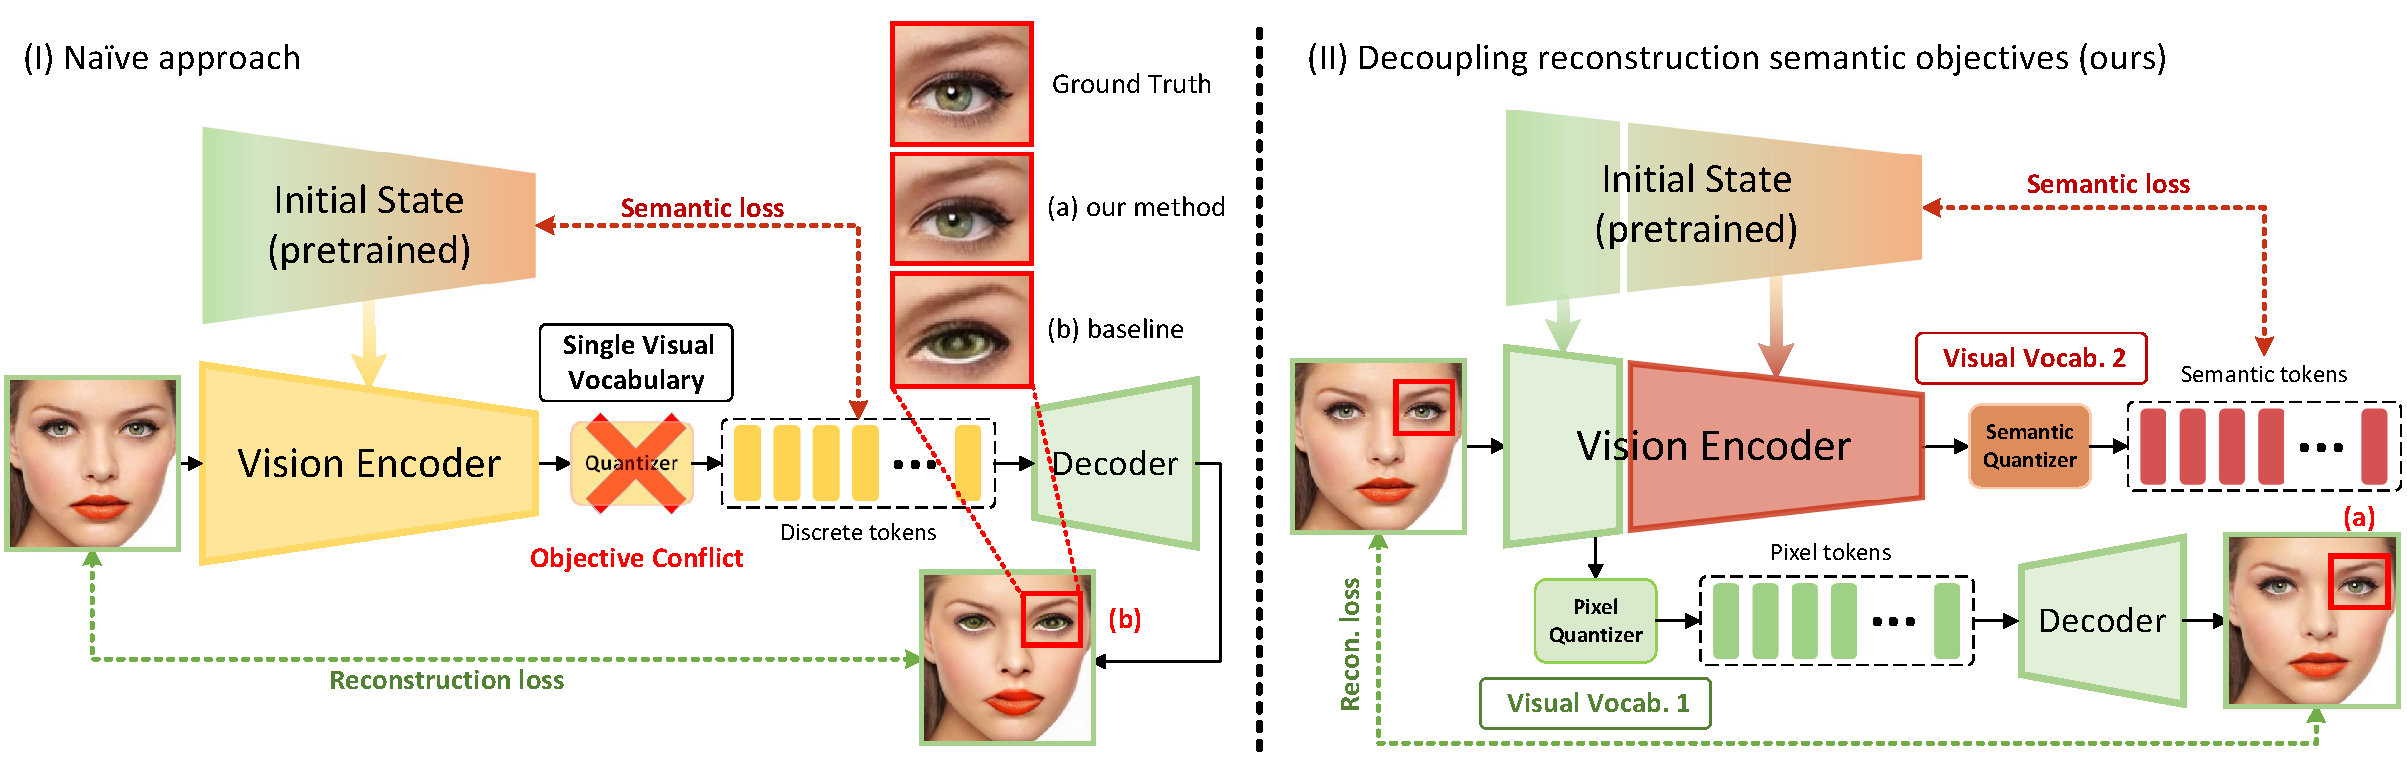
\includegraphics[width=0.475\textwidth]{imgs/tokenizer.pdf}
  \caption{
    \textbf{Comparing the design of a naive~(Left) and our decoupled approach~(Right).}
    Naively combining reconstruction and semantic loss with a single visual vocabulary leads to distorted reconstruction and degraded semantic performance. We decouple the two objectives through a hierarchy approach, where reconstruction loss is applied to supervise the shallow layers, while semantic supervision is applied to the deep layers. This enhances both reconstruction fidelity and semantic quality. Consequently, we derive two complementary visual vocabularies: a pixel codebook for low-level visual appearance, and a semantic codebook for high-level visual semantics.
    % \KY{The entire paragraph does not align with your figure. I suggest you redo this.}
  }
  \label{fig:tokenizer_framework}
  \vspace{-0.25cm}
\end{figure*}


\subsection{Unified Vision Tokenizer with Dual Codebooks}
\label{sec:method_tokenizer}

To build a unified tokenizer, we started with the simplest approach, where we directly combine the reconstruction loss and semantic loss to optimize the entire vision tower and use a single visual vocabulary to tokenize its feature, similar to VILA-U~\citep{wu2025vilau}.
Specifically, as illustrated in Fig.\ref{fig:tokenizer_framework} (left), we initialize the vision encoder with pretrained weights from SigLIP~\citep{zhai2023siglip} to ensure strong text-image alignment. Then the semantic loss is computed between the deeper-layer features of the model and its initial state to constrain the model from losing its semantic capability.

However, as shown in Table.\ref{tab:promote}~\textcolor{purple}{(a)}, this straightforward approach leads to a clear conflict between the two objectives. On one hand, although the semantic loss is applied to preserve the model's original semantic representation capabilities, achieving this objective proves difficult, as semantic performance metrics show a significant decline compared to the original model, reflecting the disruption caused by the reconstruction training objective on semantic capabilities. On the other hand, as shown in the cropped region of Fig.\ref{fig:tokenizer_framework}, the model also struggles to achieve satisfactory reconstruction quality, often producing distorted and blurry images.

\belowrulesep=0pt\aboverulesep=0pt

\begin{table}[t]
    \centering
    % \caption{\textbf{\ours{} transforms the conflict between reconstruction and semantic objectives into a positive relationship.} Directly combining the two objectives leads to a drastic decline in reconstruction performance (a vs. b). However, incorporating reconstruction and semantic losses hierarchically results in better reconstruction performance compared to using reconstruction alone (d vs. c). We \hl{highlight} our method in the last row. We adopt the pretrained weights from the siglip-so400m-patch14-384 in this experiment.
    % }
    \caption{\textbf{\ours{} resolves the conflict between reconstruction and semantic objectives.} Directly combining the two objectives leads to a drastic decline in reconstruction performance (a vs. b), while incorporating reconstruction and semantic losses hierarchically results in better reconstruction performance (a vs. d). We \hl{highlight} our method in the last row. We adopt the pretrained weights from the siglip-so400m-patch14-384 in this experiment.
    }
    \label{tab:promote}
    \tablestyle{3pt}{1.05}
    \resizebox{0.6\linewidth}{!}{
    \begin{tabular}{clccccc}
    \toprule
    \multirow{2}{*}{\# Exp.} &\multirow{2}{*}{Learning Objective (layer)}& \multirow{2}{*}{Feature Type}&\multirow{2}{*}{Zero-Shot Acc.\higherbetter} &\multicolumn{3}{c}{Reconstruction}\\ 
    \cmidrule{5-7}&&      &&rFID\lowerbetter  &PSNR\higherbetter  &SSIM\higherbetter \\
    \midrule
    \multicolumn{2}{l}{\textbf{\textit{Initial State}}}&  Continuous&83.2&\textcolor{red}{\ding{55}}  &\textcolor{red}{\ding{55}}  &\textcolor{red}{\ding{55}}  \\
    \multicolumn{2}{l}{\textbf{\textit{Initial State (quantized)}}}  &  Discrete&82.4&\textcolor{red}{\ding{55}}  &\textcolor{red}{\ding{55}}  &\textcolor{red}{\ding{55}}  \\
    ~~~~(a)~~~~~~            & Recon. (26) + Sem. (26)          &   Discrete&72.3& 3.86& 12.64&0.574\\
    ~~~~(b)~~~~~~            &Recon. (26)                      & Discrete&\textcolor{red}{\ding{55}}  &0.27&27.88&0.722\\
    ~~~~(c)~~~~~~            &Recon. (6)                       &  Discrete&\textcolor{red}{\ding{55}} & 0.29& 28.12&0.745\\
    \compare{}~~~~(d)~~~~~~  &\compare{}Recon. (6) + Sem. (26) & \compare{}Discrete&\compare{}82.0&\compare{}0.25&\compare{}28.69&\compare{}0.744\\
    \bottomrule
    \end{tabular}
    }
\end{table}

\begin{minipage}[ht]{0.425\textwidth}
    To resolve this conflict, we begin by analyzing the intrinsic properties of the SigLIP encoder. Specifically, we divide the ViT into shallow, middle, and deep layers based on the cosine similarity of features across layers, as shown in Fig.\ref{tab:cluster} (left). Guided by this partition, we extract features from the shallow and deep layer to perform clustering on the image representations. As shown in Fig.\ref{tab:cluster} (right), we observe that features from the shallow layer tend to cluster images based on low-level attributes such as color and texture, whereas features from the deep layer form clusters according to semantics. This suggests that shallow SigLIP features capture fine-grained perceptual details, while deeper layers encode high-level semantics, aligning naturally with the respective requirements of downstream visual generation and understanding tasks.
    % This suggests that shallow and deep ViT features aligns well with the respective demands of downstream generation and understanding tasks.
\end{minipage}
\hfill
\begin{minipage}[ht]{0.562\textwidth}
\vspace{0.04cm}
    \centering
    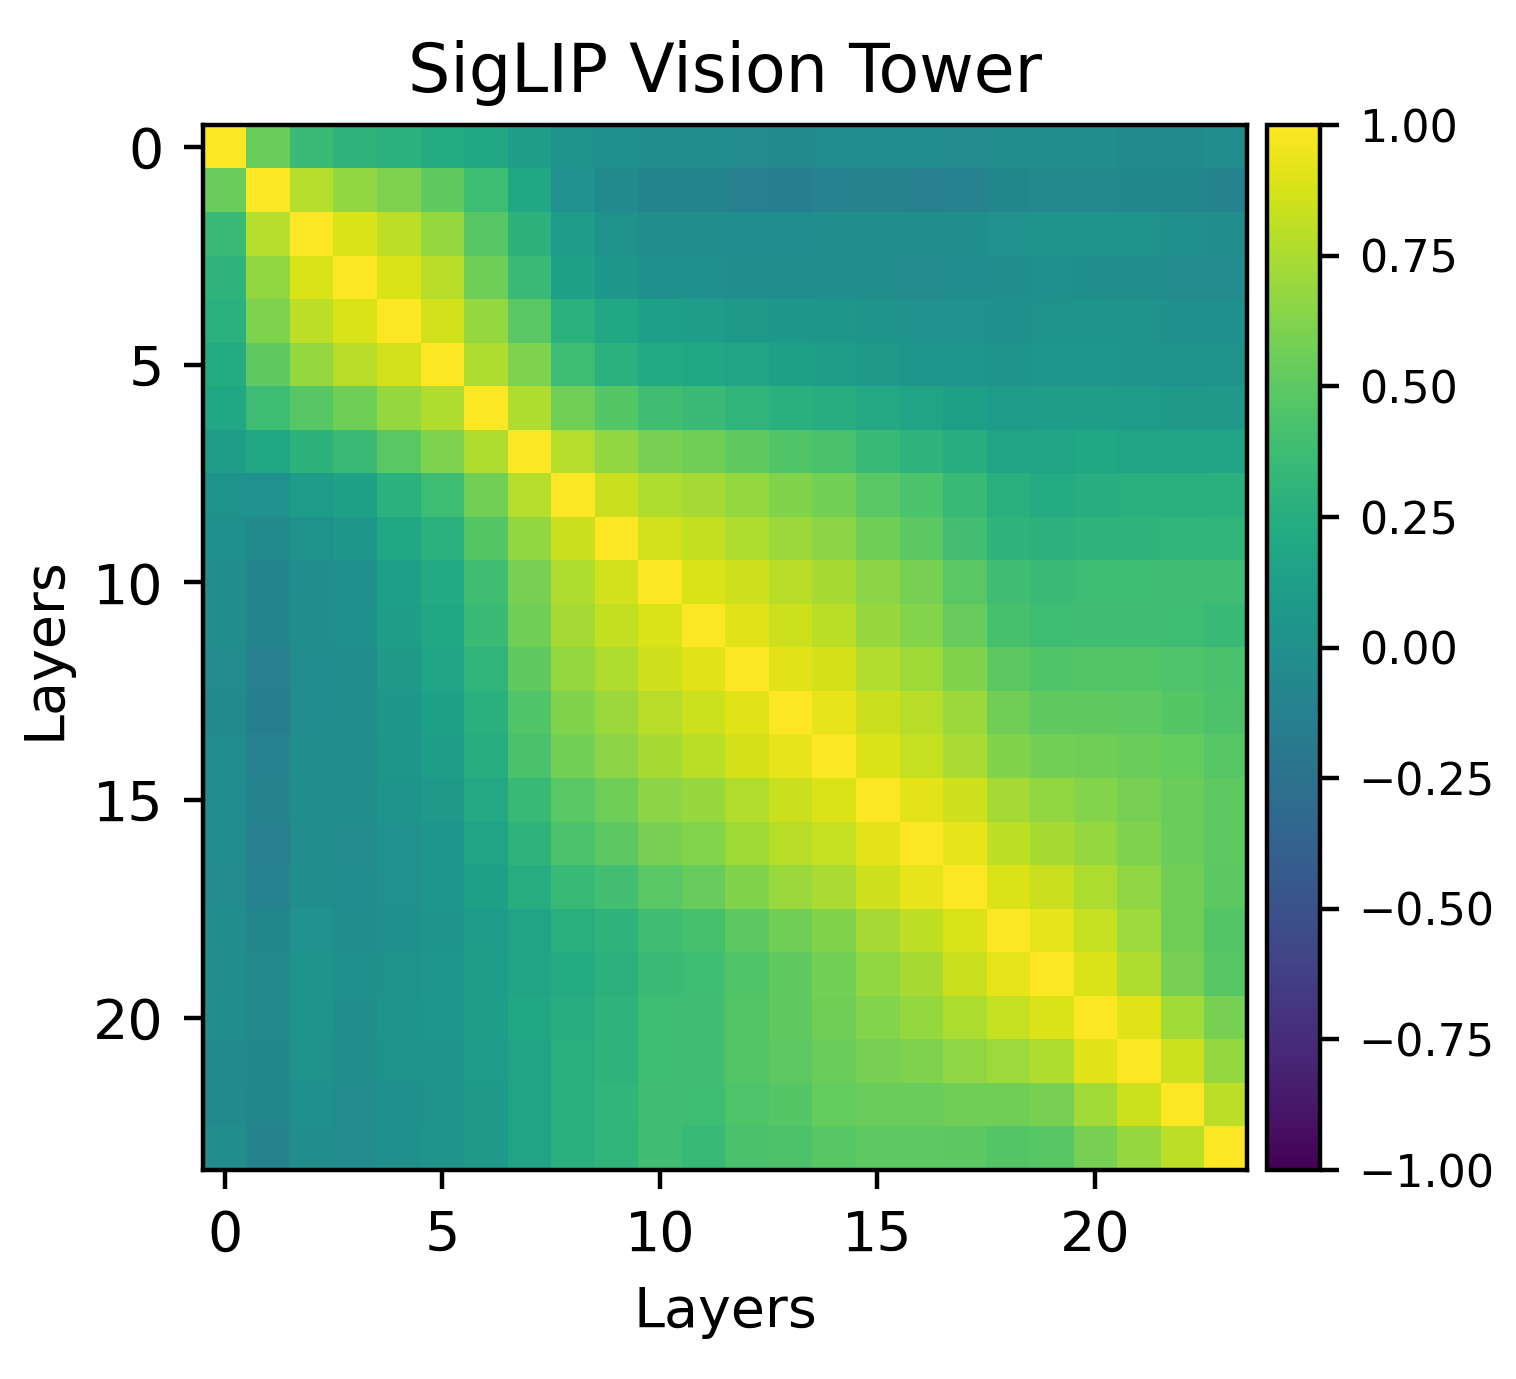
\includegraphics[height=2.13cm]{imgs/matrix_siglip.png}
    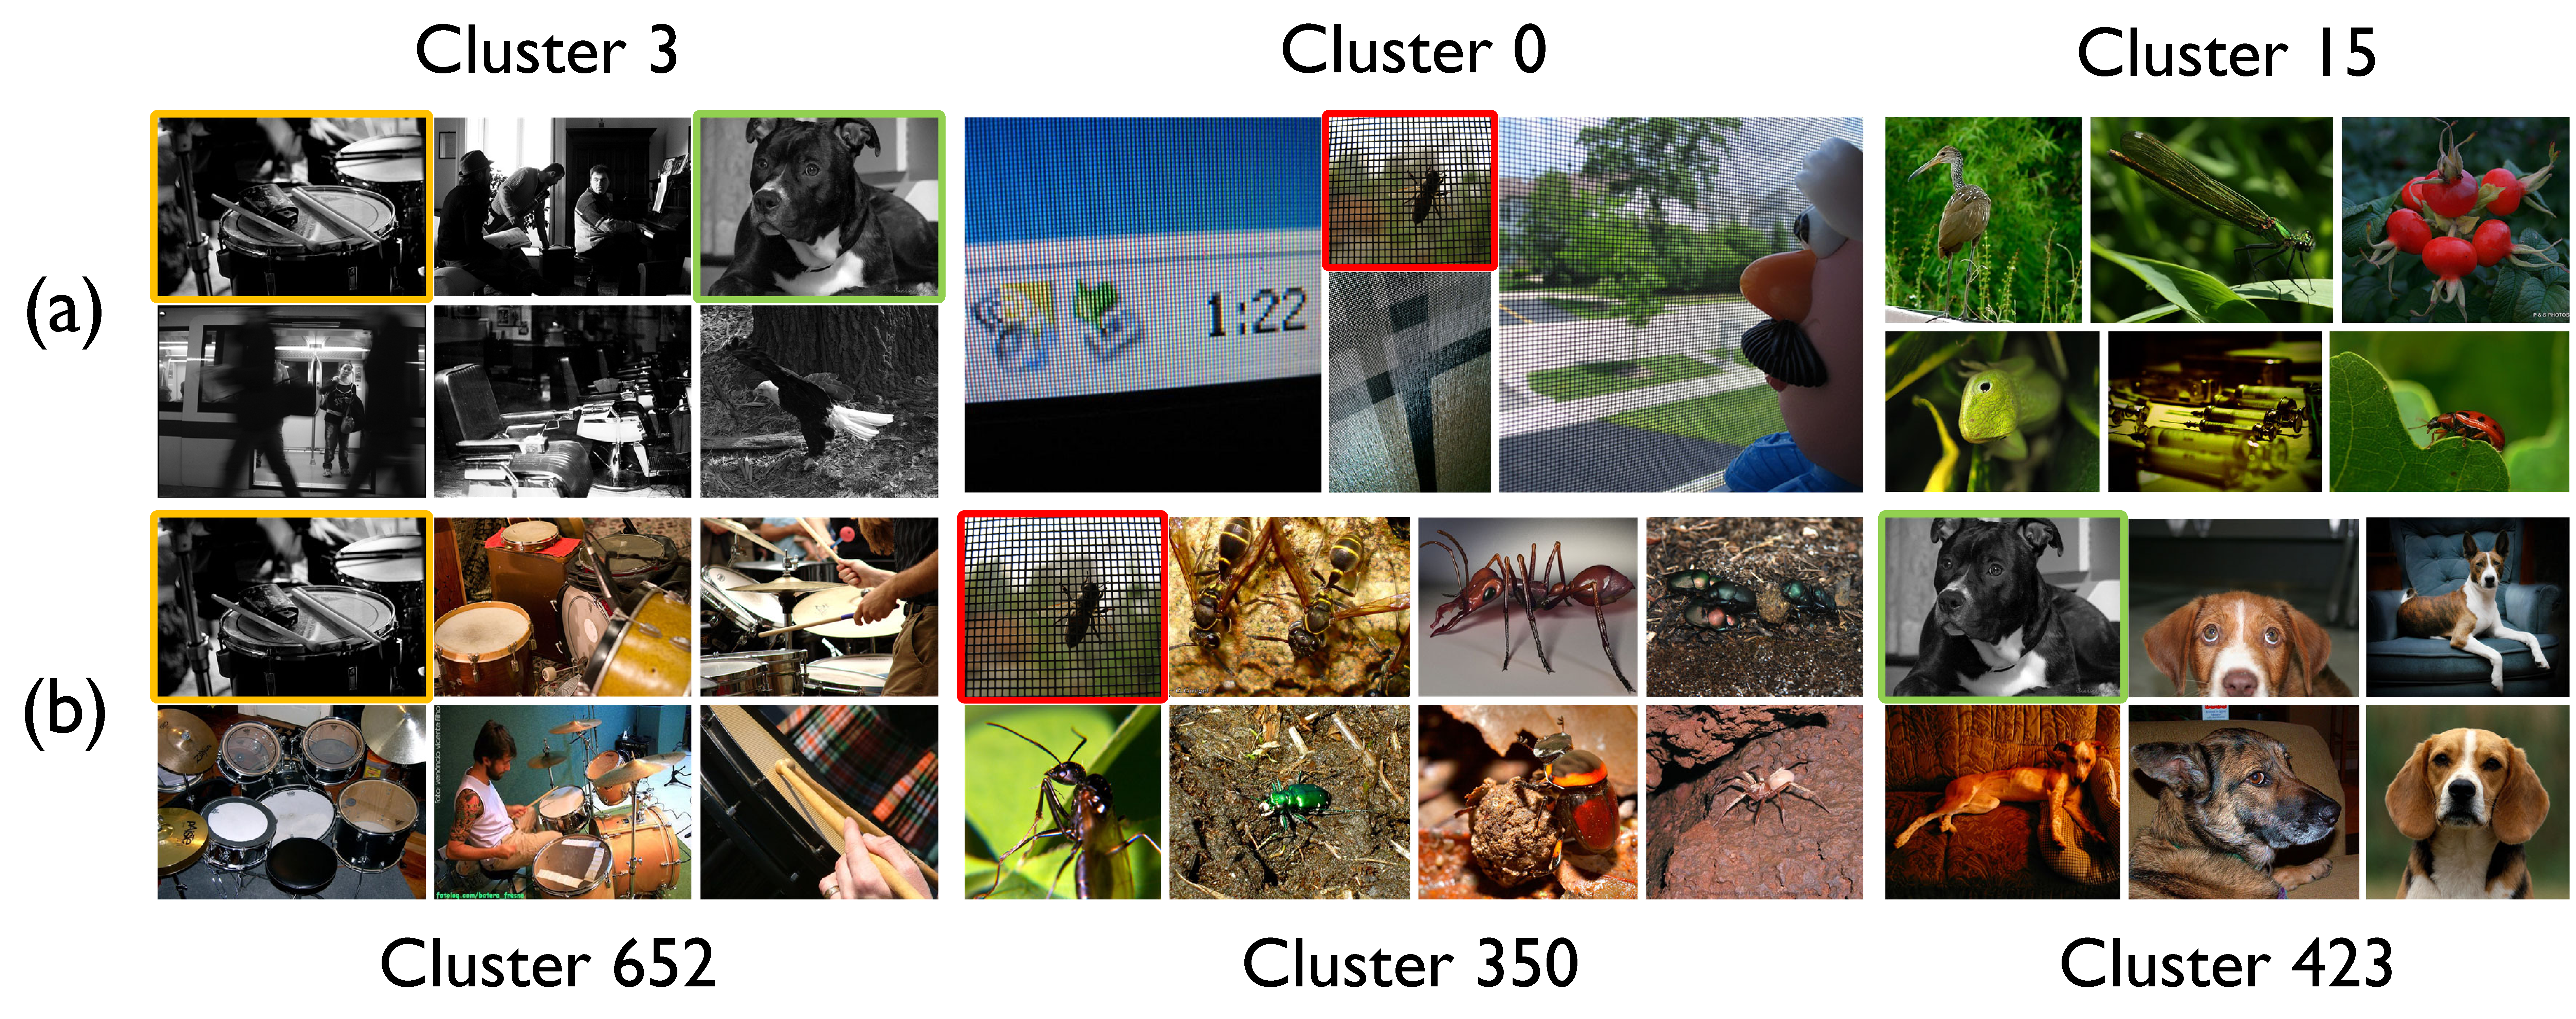
\includegraphics[height=2.13cm]{imgs/clustering-v2.pdf}
    \vspace{-0.56cm}
    \captionsetup{type=figure}
    \caption{
        \textbf{(Left)} Partitioning of the SigLIP encoder~\citep{zhai2023siglip} based on the cosine similarity of features across layers. Distinct bright square regions are observed in the ranges of layers 1–7 and 8–17, indicating strong intra-group similarity within each interval; the remaining layers are treated as deep layers.
        \textbf{(Right)} Visualization of image clusters derived from features of (a) the 6th layer and (b) the 26th layer of SigLIP. Features from deep layers cluster images based on semantic content, whereas features from shallow layers form clusters based on low-level cues such as color and texture. For example, images in cluster 0 exhibit similar grid-like textures (e.g., window screens or monitor meshes). Implementation details of the clustering process are provided in Appendix.\ref{appendix_implementation}.
    }
    \label{tab:cluster}
\end{minipage}

Motivated by this, we introduce a hierarchical approach to decouple the learning of the reconstruction and semantic objectives. Specifically, as shown in Fig.\ref{fig:tokenizer_framework} (right), reconstruction loss is applied to supervise the shallow layers (1-6) of the vision tower, while semantic loss is applied to the deep 26-th layer (Please refer to Appendix.\ref{appendix_generalizability} for the selection of the reconstruction layer).
Features from the shallow and deep layers are discretized separately via residual vector quantization~\citep{lee2022rqvae}, resulting in low-level and high-level visual vocabularies, referred to as the pixel codebook and the semantic codebook, respectively.
To ensure the encoder outputs align closely with the codebook entries, we utilize a Vector Quantization (VQ) commitment loss, which is defined as
\begin{equation}
  \mathcal{L}_{c} = \| z - \text{quantize}(z) \|_2^2
  \label{eq:loss_commit}
\end{equation}

Consequently, the total loss is formulated as a weighted sum of reconstruction loss, semantic loss, and VQ commitment loss
\begin{equation}
  \mathcal{L}_{total} = \lambda_1 \cdot \mathcal{L}_{recon} + \lambda_2 \cdot \mathcal{L}_{sem} +  \lambda_3 \cdot (\mathcal{L}_{c1} + \mathcal{L}_{c1})
  \label{eq:loss_total}
\end{equation}

where the reconstruction loss is the combination of pixel-wise $L2$ loss \citep{dosovitskiy2016L2}, LPIPS loss \citep{zhang2018lpips} and adversarial loss \citep{isola2017gan} for reconstructing an input image
\begin{equation}
\begin{aligned}
  \mathcal{L}_{recon} = \|\hat{x} - x\|_2^2 + \lambda_p\mathcal{L}_{\text{LPIPS}}(\hat{x},x) + \lambda_g\mathcal{L}_{\text{G}}(\hat{x})
  \label{eq:loss_recon}
\end{aligned}
\end{equation}

% while the semantic loss is simply computed as the $L_2$ distance between the model's last-layer feature $F$ and its initial value $F_0$
while the semantic loss is computed as the distance between the model's final-layer feature $F$ and its initial value $F_0$
\begin{equation}
\begin{aligned}
  \mathcal{L}_{sem} = -\mathrm{cos}(F, F_0) + \|F - F_0\|_2^2
  \label{eq:loss_sem}
\end{aligned}
\end{equation}

where $\mathrm{cos}(\cdot)$ denotes cosine similarity. Interestingly, as shown in Table.\ref{tab:promote} \textcolor{purple}{(d)}, even without adding an additional contrastive learning phase, but solely by applying a simple constraint on the semantic representation, incorporating a reconstruction objective within our hierarchical learning strategy causes minimal damage to the model's semantic capability.
Moreover, as shown in Table.\ref{tab:promote} \textcolor{purple}{(b)(c)(d)}, compared to training solely for reconstruction, incorporating semantic supervision in the deeper layers does not degrade reconstruction performance in the shallow layers, effectively resolving the conflict between semantic and reconstruction objectives.


\subsection{Unifying Understanding and Generation}
\label{sec:method_mllm}


\begin{figure*}[t]
  \centering
  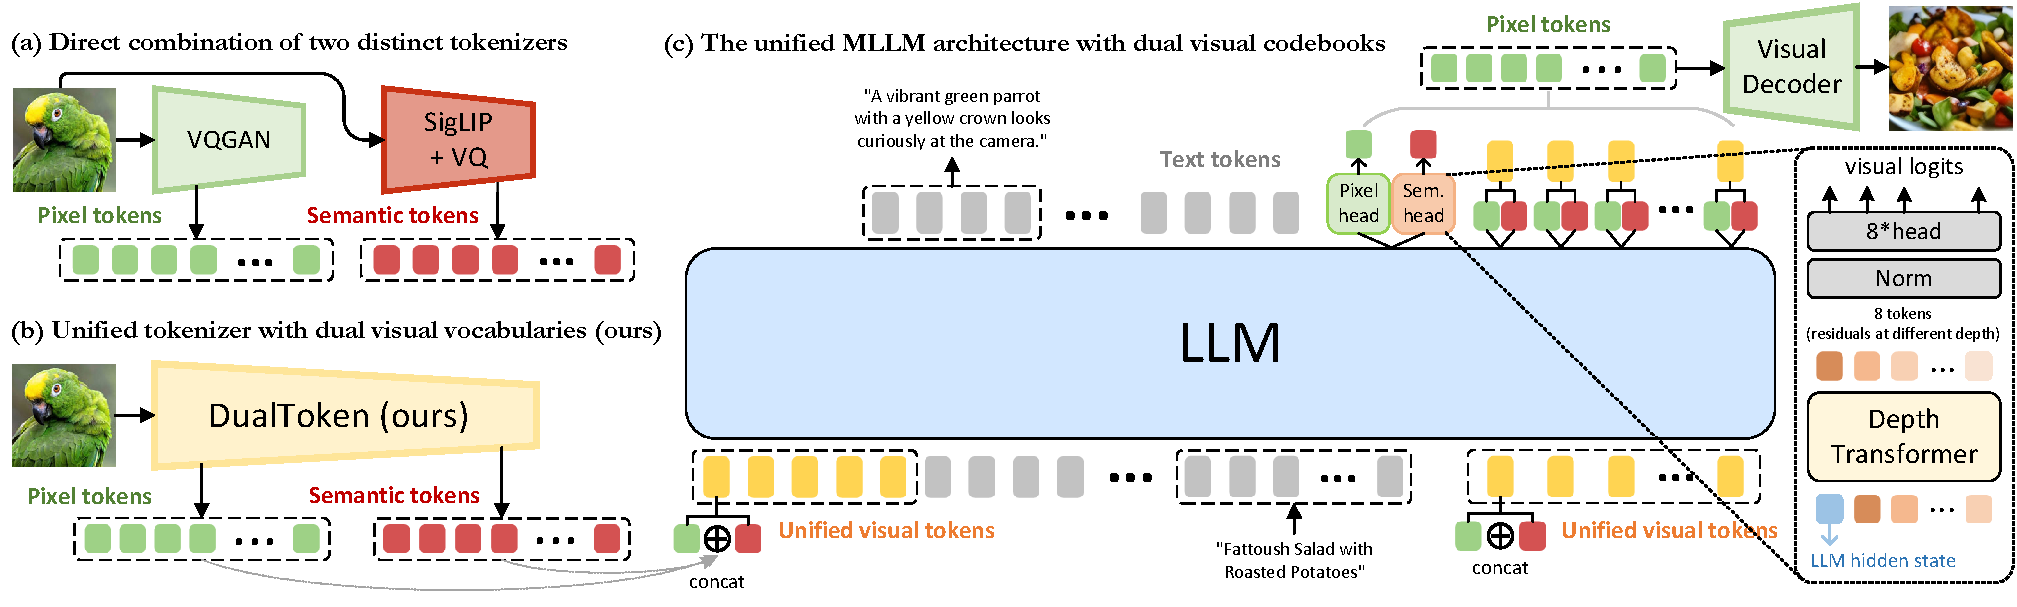
\includegraphics[width=\textwidth]{imgs/frameworks-v4.pdf}
  \caption{
      % \textbf{
      % (Left) Comparing directly 
      % An overview of our framework utilizing dual visual codebooks for unified visual understanding and generation.
      % }
      \textbf{(a) Direct combination of two heterogeneous tokenizer.} Baseline method~\citep{huang2025illume+} that directly uses VQGAN and CLIP-based encoder to separately acquire high-level (semantic) and low-level (pixel) visual codebooks.
      \textbf{(b) Our unified tokenizer with dual codebook.} We decoupling high-level and low-level visual codebooks within a unified vision tokenizer. The image is converted into low-level visual appearance tokens (green) and text-aligned semantic tokens (red).
      \textbf{(c) Architecture for unifying generation and understanding task.} % To model both textual and visual modality within the autoregressive paradigm, the pixel and semantic visual tokens are concatenated along their embedding dimension to form unified visual tokens (yellow). These unified visual tokens are then concatenated with text tokens to construct a multimodal token sequence.
      % The high-level and low-level visual tokens are predicted by independent visual heads (Pixel head and Semantic head).
      In image generation task, the generated low-level tokens are decoded by the visual decoder to reconstruct the visual content.
  }
  \label{fig:frameworks}
  % \vspace{-20pt}
\end{figure*}


In this section, we demonstrate how to integrate the dual visual codebooks of \ours{} within a unified MLLM.
As illustrated in Fig.\ref{fig:frameworks} \textcolor{purple}{(c)}, to model both textual and visual content within the autoregressive paradigm of LLMs, the pixel and semantic visual tokens are first passed through a 2-layer MLP projector to align their dimensions with the LLM backbone. These tokens are then concatenated \textbf{along the embedding dimension} (which does not increase the sequence length) to form unified visual tokens. Next, the unified visual tokens are concatenated with text tokens to construct a multimodal token sequence. The model is then trained in an autoregressive manner to predict the next token across both visual and textual content.

For simplicity, we define the language vocabulary of our MLLM as a finite set $\mathcal{X}=\{x_1, x_2, ..., x_{n_1}\}$, while the low-level and high-level visual vocabulary as $\mathcal{Y}=\{y_1, y_2, ..., y_{n_2}\}$ and $\mathcal{Z}=\{z_1, z_2, ..., z_{n_3}\}$, where $n_1$, $n_2$, and $n_3$ represent the vocabulary sizes for language tokens, low-level visual tokens, and high-level visual tokens, respectively.

For visual tokens, since residual quantization introduces a depth-stacked structure of codes at each visual position $p$, we implement our visual heads based on the depth transformer from RQ-VAE \citep{lee2022rqvae}. 
% Unlike the original depth transformer, which employs a single head to predict logits across all depths, we introduce separate classification heads to compute the logits for residuals at each corresponding depth \citep{li2025baichuanaudio}.
As shown in Fig.\ref{fig:frameworks}, the semantic tokens and pixel tokens are processed by independent visual heads---the pixel head and the semantic head. Both heads share the same structure, comprising three layers of depth transformers and corresponding classification head for each depth.

Given the LLM hidden state $h_p$ for visual tokens at position $p$, our depth transformer autoregressively predicts D residual tokens ($r_{p1}$, $r_{p2}$, ..., $r_{pD}$). For $d > 1$, the input to the depth transformer at depth d, denoted as $I_{pd}$, is defined as the sum of the token embeddings of up to depth $d-1$ 
\begin{equation}
\begin{aligned}
  I_{pd} = \sum_{d'=1}^{d-1} \mathbf{e}(r_{pd'}),
\end{aligned}
\end{equation}
where $r\in\mathcal{Y}$ for the pixel head and $r\in\mathcal{Z}$ for the semantic head. The initial input at depth 1 is given by $I_{p1} = h_p$. This formulation ensures that the depth transformer incrementally refines the predicted feature representation by leveraging previous estimations up to depth $d-1$.
Consequently, the overall negative log-likelihood loss for the entire multimodal sequence of length $N$ is defined, if a text token appears at position $i$, as
\begin{equation}
\begin{aligned}
  \mathcal{L}_\text{NTP} = -\sum_{i=1}^N\mathcal{P}_i, 
\text{, where } \mathcal{P}_i = \log P\left(x_i|x_{<i}\right)
\end{aligned}
\end{equation}
% \begin{equation}
% \begin{aligned}
%     \mathcal{P}_i = \log P\left(x_i|x_{<i}\right)
% \end{aligned}
% \vspace{0.15cm}
% \end{equation}
 and if visual tokens appears at position $i$, as
\begin{equation}
\begin{aligned}
    \mathcal{P}_i = \sum_{d=1}^D~[\log P\left(y_{id}|y_{i,<d}\right)+\log P\left(z_{id}|z_{i,<d}\right)]
\end{aligned}
\end{equation}

% During multimodal pretraining, the weights of the depth transformers are randomly initialized and trained jointly with the LLM.
% During inference, only the pixel tokens are utilized by the visual decoder to reconstruct the visual content.
% \vspace{-2mm}